\documentclass[10pt, a4paper]{article}

\usepackage[english]{babel}
\usepackage[margin=2cm, nohead]{geometry}
\usepackage{parskip}
\usepackage{listings}
\usepackage{array}
\usepackage{arydshln}
\usepackage[T1]{fontenc}
\usepackage{amsmath}
\usepackage{graphicx}
\usepackage{tikz}
\usetikzlibrary{shapes,fit}

\begin{document}

\begin{center}
\LARGE Block Heap Layout
\end{center}

\section{Abstract}

In this document I will present an alternative memory layout for binary heaps called block heap layout (BHL).
In a $d$-BHL subtrees of height $d$ are stored continuously opposed to the standard layout for binary trees which stores nodes layer by layer.
I will first define the BHL structure and then analyse it in comparison to the standard binary tree layout.

\section{Definition}

The following illustration represents one block in the $d$-BHL structure (the number in the node refers to its position when saved in the array):

\begin{tikzpicture}[level/.style={sibling distance=3cm/#1,level distance=1cm}]
\node [rectangle,draw] (n0){0}
	child {node [rectangle,draw] (n1) {1}
		child {node{$\vdots$}
			child {node [rectangle,draw] (n3) {$2^d-1$}}
			child {node {} edge from parent[draw=none]}
		}
		child {node{$\vdots$}}
	}
	child {node [rectangle,draw] (n2) {2}
		child {node{$\vdots$}}
		child {node{$\vdots$}
			child {node {} edge from parent[draw=none]}
			child {node [rectangle,draw] (n4) {$2^{d+1}-2$}}
		}
	};
    
\path (n3) -- (n4) node [midway] {$\cdots$};
\end{tikzpicture}

In order to use the BHL structure for heaps of any size, we can make each of the $2^{d+1}$ children of leafs in a block root nodes of another block:

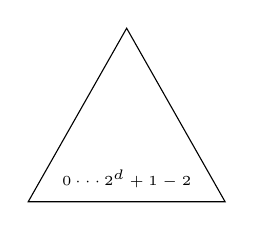
\begin{tikzpicture}[
	leaf/.style={isosceles triangle,draw,shape border rotate=90,isosceles triangle stretches=true, minimum height=15mm,minimum width=25mm,inner sep=0,yshift={-20mm},font=\tiny}
]
\node[leaf] {$0\cdots 2^d+1 - 2$};
\end{tikzpicture}

\end{document}